%%%%%%%%%%%%%%%%%%%%%%%%%%%%%%%%%%%%%%%%%
% Beamer Presentation
% LaTeX Template
% Version 1.0 (10/11/12)
%
% This template has been downloaded from:
% http://www.LaTeXTemplates.com
%
% License:
% CC BY-NC-SA 3.0 (http://creativecommons.org/licenses/by-nc-sa/3.0/)
%
%%%%%%%%%%%%%%%%%%%%%%%%%%%%%%%%%%%%%%%%%

%----------------------------------------------------------------------------------------
%	PACKAGES AND THEMES
%----------------------------------------------------------------------------------------

\documentclass{beamer}

\mode<presentation> {

% The Beamer class comes with a number of default slide themes
% which change the colors and layouts of slides. Below this is a list
% of all the themes, uncomment each in turn to see what they look like.

%\usetheme{default}
%\usetheme{AnnArbor}
%\usetheme{Antibes}
%\usetheme{Bergen}
%\usetheme{Berkeley}
%\usetheme{Berlin}
%\usetheme{Boadilla}
%\usetheme{CambridgeUS}
%\usetheme{Copenhagen}
%\usetheme{Darmstadt}
%\usetheme{Dresden}
\usetheme{Frankfurt}
%\usetheme{Goettingen}
%\usetheme{Hannover}
%\usetheme{Ilmenau}
%\usetheme{JuanLesPins}
%\usetheme{Luebeck}
%\usetheme{Madrid}
%\usetheme{Malmoe}
%\usetheme{Marburg}
%\usetheme{Montpellier}
%\usetheme{PaloAlto}
%\usetheme{Pittsburgh}
%\usetheme{Rochester}
%\usetheme{Singapore}
%\usetheme{Szeged}
%\usetheme{Warsaw}

% As well as themes, the Beamer class has a number of color themes
% for any slide theme. Uncomment each of these in turn to see how it
% changes the colors of your current slide theme.

%\usecolortheme{albatross}
%\usecolortheme{beaver}
%\usecolortheme{beetle}
%\usecolortheme{crane}
%\usecolortheme{dolphin}
%\usecolortheme{dove}
%\usecolortheme{fly}
%\usecolortheme{lily}
%\usecolortheme{orchid}
%\usecolortheme{rose}
%\usecolortheme{seagull}
%\usecolortheme{seahorse}
%\usecolortheme{whale}
%\usecolortheme{wolverine}

%\setbeamertemplate{footline} % To remove the footer line in all slides uncomment this line
\setbeamertemplate{footline}[page number] % To replace the footer line in all slides with a simple slide count uncomment this line

\setbeamertemplate{navigation symbols}{} % To remove the navigation symbols from the bottom of all slides uncomment this line
}

\usepackage{graphicx} % Allows including images
\usepackage{booktabs} % Allows the use of \toprule, \midrule and \bottomrule in tables
\usepackage[brazil]{babel}
\usepackage{amsmath}
\usepackage{multirow}
\usepackage[version=4]{mhchem}
\usepackage{caption}
\usepackage{subcaption}
\usepackage{tikz}
\usepackage{xcolor}

%----------------------------------------------------------------------------------------
%	TITLE PAGE
%----------------------------------------------------------------------------------------

\title[Redes Neurais Artificiais 2020/2]{Maximização de Margem} % The short title appears at the bottom of every slide, the full title is only on the title page

\author{Victor Ruela} % Your name
\institute[PPGEE - UFMG] % Your institution as it will appear on the bottom of every slide, may be shorthand to save space
{
Programa de Pós-Graduação em Engenharia Elétrica\\ Universidade Federal de Minas Gerais \\ % Your institution for the title page
\medskip
\textit{victorspruela@ufmg.br} % Your email address
}
\date{\today} % Date, can be changed to a custom date

%\setbeamertemplate{sidebar right}{}
%\setbeamertemplate{footline}{%
%	\hfill\usebeamertemplate***{navigation symbols}
%	\hspace{1cm}\insertframenumber{}/\inserttotalframenumber}


%\AtBeginSection[]
%{
%	\begin{frame}
%		\frametitle{Agenda}
%		\tableofcontents[currentsection,currentsubsection]
%	\end{frame}
%}

\begin{document}

\begin{frame}
\titlepage % Print the title page as the first slide
\end{frame}

\begin{frame}
\frametitle{Agenda} % Table of contents slide, comment this block out to remove it
\tableofcontents % Throughout your presentation, if you choose to use \section{} and \subsection{} commands, these will automatically be printed on this slide as an overview of your presentation
\end{frame}

%----------------------------------------------------------------------------------------
%	PRESENTATION SLIDES
%----------------------------------------------------------------------------------------

%------------------------------------------------
\section{Introdução} % Sections can be created in order to organize your presentation into discrete blocks, all sections and subsections are automatically printed in the table of contents as an overview of the talk
%------------------------------------------------

%\subsection{Aprendizado Supervisionado}

\begin{frame}
	\frametitle{Definição do Problema}
	\begin{itemize}
		\item Dados de treinamento: $\mathcal{T} = \left\lbrace (\textbf{x}_1, d_1), \dots, (\textbf{x}_N, d_N)\right\rbrace $
		\item Problema de classificação binário: $d_i = \{ -1, 1 \} $
		\item Linearmente separável
		\item Existem infinitos hiperplanos separadores!
%		\item Em geral, algoritmos para treinamento de RNAs objetivam minimizar o erro quadrático:
%		\begin{equation}
%			\min \sum_{i=1}^{N} [d_i - sign(\textbf{w}^T\textbf{x}_i + b)]^2
%			\label{eq:sqrd}
%		\end{equation}
		
	\end{itemize}
	\begin{figure}[h!]
		\centering
		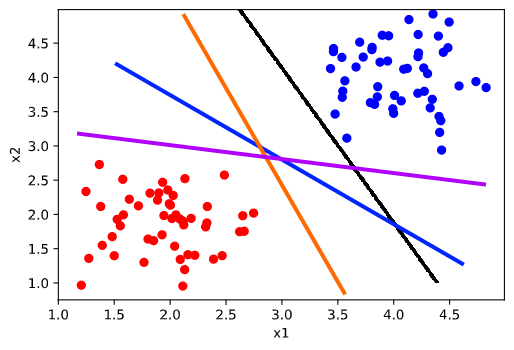
\includegraphics[width=3.0in]{fig01_01.png}
		\label{fig:plano-mse}
	\end{figure}
%	\begin{figure}[h!]
%		\centering
%		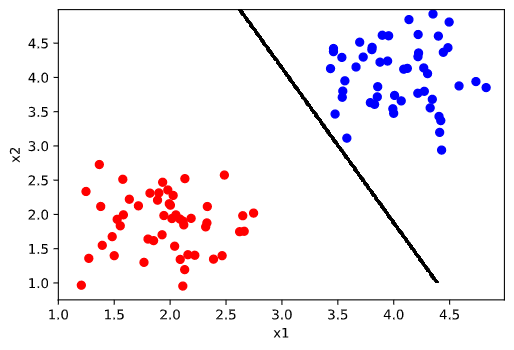
\includegraphics[width=3.0in]{fig01.png}
%	\end{figure}

\end{frame}

%\subsection{Minimização do Erro}

\begin{frame}
	\frametitle{Definição do Problema}
	\begin{itemize}
		\item O uso do Perceptron, por exemplo, encontrará um hiperplano que separa estes padrões:
		\begin{equation}
	 		g(\textbf{x}) = \textbf{w}^T\textbf{x} + b = 0
	 		\label{eq:plano}
 		\end{equation}
 		\item Entretanto, considerar a distância de todos os pontos para treinamento não é uma garantia de otimalidade
		\item E se fossem usados somente aqueles mais difíceis de serem separados e próximos da superfície de separação?
		
		\begin{block}{Maximização de Margem}
			Abordagem introduzida por Vapnik \cite{vapnik} para encontrar uma superfície de separação ótima com boa generalização, aplicável a diferentes modelos lineares
		\end{block}		

	\end{itemize}

\end{frame}

\section{Maximização de Margem}

\subsection{O Hiperplano Ótimo}


%\begin{frame}
%	\frametitle{O Hiperplano Ótimo}
%	\begin{columns}
%		\begin{column}{0.5\textwidth}  
%			\begin{center}
%				\begin{itemize}
%					\item A função discriminante ótima é definida como:
%					\begin{equation}
%						g(\textbf{x}) = \textbf{w}^T_o\textbf{x} + b_o
%						\label{eq:plano-opt}
%					\end{equation}		
%					\item E a distância deste hiperplano por:
%					\begin{equation}
%						r = \frac{g(\textbf{x})}{\left \| \textbf{w}_o \right \|} 
%						\label{eq:plano-dist}
%					\end{equation}		
%				\end{itemize}
%			\end{center}
%		\end{column}
%		\begin{column}{0.5\textwidth}
%			\begin{figure}[h!]
%				\centering
%				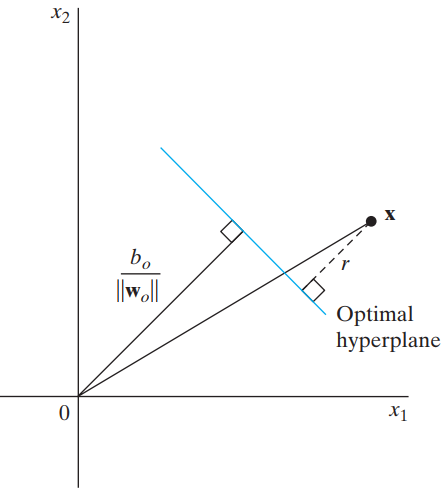
\includegraphics[width=2in]{fig04.png}
%				\label{fig:haykin-03}
%			\end{figure}
%		\end{column}
%	\end{columns}
%\end{frame}


\begin{frame}
	\frametitle{O Hiperplano Ótimo}
	\begin{itemize}
		\item Quando a escolha de $\textbf{w}$ e $b$ maximizam a margem de separação ($\rho$), o hiperplano é dito \textbf{ótimo} \cite{haykin}:
		\begin{equation}
			\textbf{w}^T_o\textbf{x} + b_o = 0
			\label{eq:plano-opt}
		\end{equation}		

		\item Para otimalidade, o par ($\textbf{w}_o$,$b_o$) deve satisfazer:
		\begin{equation}
		\begin{cases}
			\textbf{w}^T_o\textbf{x}_i \geq 1, & d_i = +1 \\ 
			\textbf{w}^T_o\textbf{x}_i \leq -1, & d_i = -1
		\end{cases}
		\label{eq:plano-cond}
		\end{equation}
		\item Os pontos ($\textbf{x}_i$,$d_i$) que satisfazem com igualdade estas restrições são chamados de \textbf{vetores de suporte}
		\item Eles são os pontos mais próximos do hiperplano e consequentemente mais difíceis de classificar \cite{haykin}.
	\end{itemize}

\end{frame}

\begin{frame}
	\frametitle{O Hiperplano Ótimo}
	\begin{figure}[h!]
		\centering
		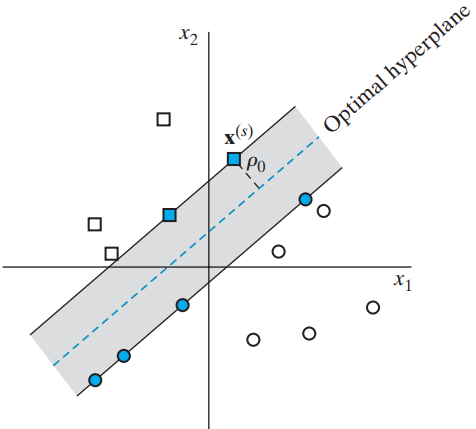
\includegraphics[width=0.6\textwidth]{fig03.png}
		\caption{Representação do hiperplano ótimo e seus elementos. Extraído de \cite{haykin}}
		\label{fig:haykin-01}
	\end{figure}
\end{frame}


\begin{frame}
	\frametitle{O Hiperplano Ótimo}
	
	\begin{itemize}
		\item Pela definição do vetor de suporte $\textbf{x}^{(s)}$:
		\begin{equation}
			g(\textbf{x}^{(s)})=\textbf{w}^T_o\textbf{x}^{(s)} + b_o = \mp 1
			\label{eq:support-vectors}
		\end{equation}	
		\item Logo, sua distância ao hiperplano separador é dada por:
		\begin{eqnarray}
		r &=& \frac{g(\textbf{x}^{(s)})}{\left \| \textbf{w}_o \right \|} \\
		  &=& \begin{cases}
			\frac{1}{\left \| \textbf{w}_o \right \|} & \text{ se } d^{(s)}= +1\\ 
			\frac{-1}{\left \| \textbf{w}_o \right \|}& \text{ se } d^{(s)}= -1 
		\end{cases}
		\end{eqnarray}
		\item Finalmente, a margem ótima $\rho$ é:
		\begin{equation}
			\rho = \frac{2}{\left \| \textbf{w}_o \right \|}
			\label{eq:margin-opt}
		\end{equation}
	\end{itemize}	
	
	\begin{block}{Conclusão}
		Maximizar a margem de separação entre classes binárias é equivalente a minimizar a norma Euclidiana do vetor de pesos $\textbf{w}$
	\end{block}

\end{frame}


%\begin{frame}
%	\frametitle{O Hiperplano Ótimo}
%
%		\begin{figure}[h!]
%			\centering
%			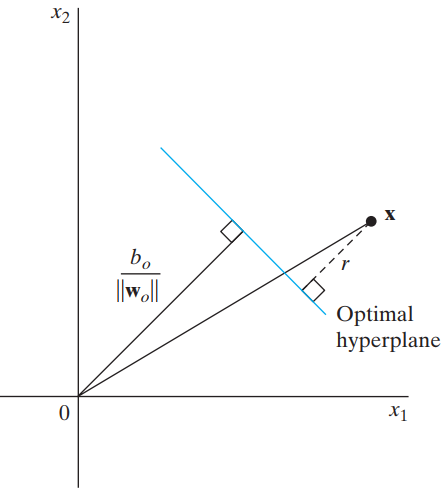
\includegraphics[width=0.5\textwidth]{fig04.png}
%			\caption{Distância de um ponto ao hiperplano ótimo. Extraído de \cite{haykin}}
%			\label{fig:haykin-03}
%		\end{figure}
%
%\end{frame}

%\subsection{Padrões Linearmente Separáveis}

\subsection{Solução}

\begin{frame}
	\frametitle{Formulação do Problema}
	\begin{itemize}
		\item Combinando as Equações (\ref{eq:support-vectors}) e (\ref{eq:margin-opt}), podemos formular o problema de encontrar a margem ótima como:
		\begin{align}
			\underset{\textbf{w},b}{\text{minimizar}} \quad & \frac{1}{2}\textbf{w}^T\textbf{w} \\ 
			\text{sujeito a} \quad & d_i(\textbf{w}^T\textbf{x}_i + b) \geq 1, \quad i=1,2,\dots,N  \nonumber
			\label{eq:opt-prob1}
		\end{align} 
		\item Problema com objetivo quadrático e restrições lineares. 
		\item Por ser convexo, possuirá solução única.
		\item É reformulado e resolvido através da técnica de multiplicadores de Lagrange \cite{haykin}
		\item Mais fácil de ser reolvido e fornece os vetores de suporte
		
	\end{itemize}
	
\end{frame}

\begin{frame}
	\frametitle{Resultado}
	\begin{figure}[h!]
		\centering
		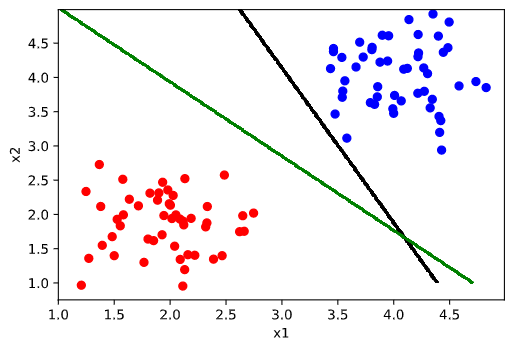
\includegraphics[width=3in]{fig02.png}
		\caption{Superfícies de separação: MSE (preta) e margem máxima (verde)}
		\label{fig:opt-margin-ds}
	\end{figure}
\end{frame}

\subsection{Padrões Não Separáveis}
\begin{frame}
	\frametitle{Padrões Não Separáveis}
	\begin{itemize}
		\item Em aplicações práticas, não podemos garantir que os dados sejam perfeitamente separáveis
		\item Logo, é adicionada uma variável de folga $\xi$ para representar estas discrepâncias:
		\begin{align}
			\underset{\textbf{w},b}{\text{minimizar}} \quad & \frac{1}{2}\textbf{w}^T\textbf{w} + \textcolor{red}{C\sum_{i=1}^{N}\xi_i} \\ 
			\text{sujeito a} \quad & d_i(\textbf{w}^T\textbf{x}_i + b) \geq 1 \textcolor{red}{- \xi_i} \quad i=1,2,\dots,N   \nonumber \\
			& \textcolor{red}{\xi_i \geq 0} \nonumber
		\end{align} 
		\item É reformulado e resolvido de forma similar ao Problema (\ref{eq:opt-prob1})
		\item A constante $C$ controla a generalização do modelo
		\item Deve ser definida usando validação cruzada, por exemplo
	\end{itemize}
	
\end{frame}


\section{Problemas não-linearmente separáveis}
\begin{frame}
	\frametitle{Problemas não-linearmente separáveis}
	\begin{itemize}
		\item Problemas reais nem sempre podem ser separados linearmente
		\item Entretanto, podemos mapeá-lo para um novo espaço de alta dimensão onde ele é mais provável de ser linearmente separável: \textbf{Teorema de Cover} \cite{cover}
		\item Este mapeamento é feito por funções não-lineares conhecidas como \textit{Kernels}
	\end{itemize}
	\begin{figure}[h!]
		\centering
		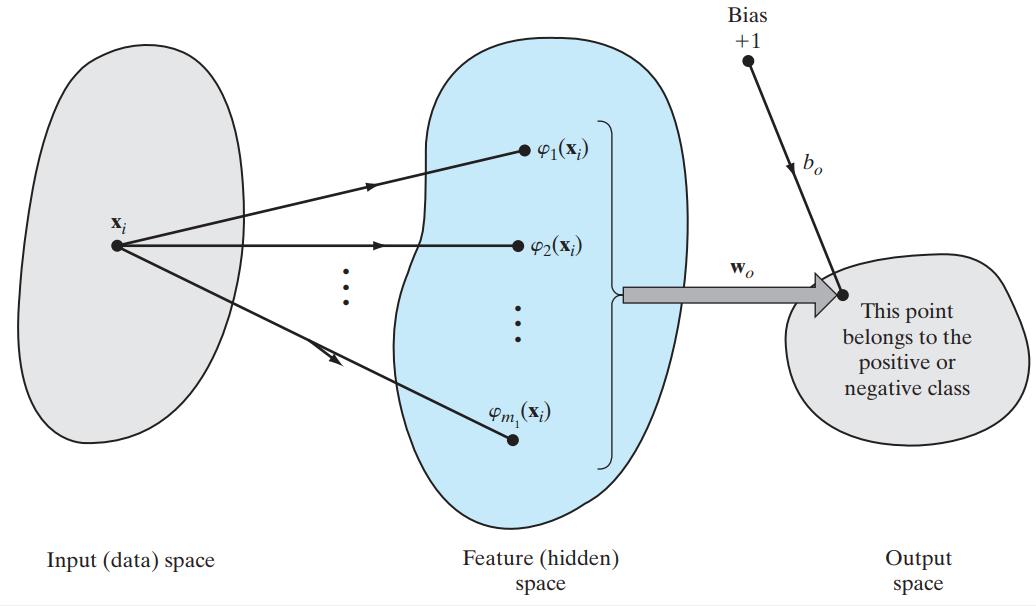
\includegraphics[width=3in]{fig05.png}
		\label{fig:kernel-trick}
	\end{figure}
\end{frame}

\begin{frame}
	\frametitle{Truque do Kernel}
	\begin{itemize}
		\item No espaço original (primal):
		\begin{equation}
	 		g(\textbf{x})^p = \textbf{w}^T.\varphi(\textbf{x}) + b
	 		\label{eq:primal}
		\end{equation}
		\item Após a transformação para o espaço dual:
		\begin{equation}
			g(\textbf{x})^d = \sum_{k=1}^{N} \alpha_kK(\textbf{x}_k,\textbf{x}) + b
	 		\label{eq:dual}
		\end{equation}
		\item Escolhendo um Kernel apropriado \cite{mercer}, as Equações (\ref{eq:primal}) e (\ref{eq:dual}) são representações duais da mesma superfície de decisão, portanto:
		\begin{equation}
		 	w_i = \sum_{k=1}^{N} \alpha_k\varphi_i(\textbf{x}_k)
			\label{eq:rela}
		\end{equation}
	\end{itemize}
\end{frame}


\subsection{Exemplos}
\begin{frame}
	\frametitle{Exemplo - SVM}
	\begin{columns}
		\begin{column}{0.5\textwidth}  
			\begin{figure}
				\centering
				\begin{subfigure}[h!]{1\textwidth}
					\centering
					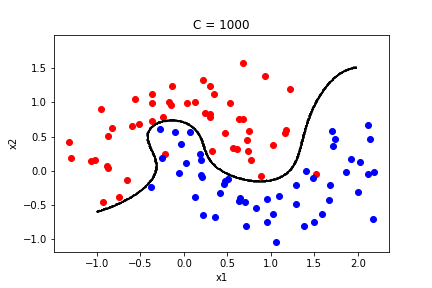
\includegraphics[width=\linewidth]{fig08.png}
					\label{fig:c-1000}
				\end{subfigure}
				\begin{subfigure}[h!]{1\textwidth}
					\centering
					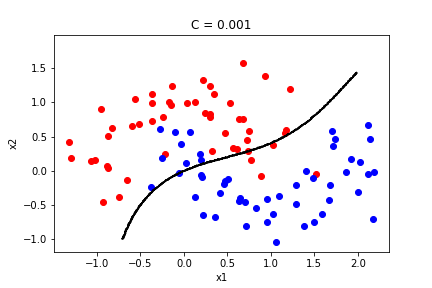
\includegraphics[width=\linewidth]{fig09.png}
					\label{fig:c-0.001}
				\end{subfigure}
				%\caption{Variação da constante de regularização $C$}
				\label{fig:reg-C}
			\end{figure}
		\end{column}
		\begin{column}{0.5\textwidth}
			\begin{figure}
				\centering
				\begin{subfigure}[h!]{1\textwidth}
					\centering
					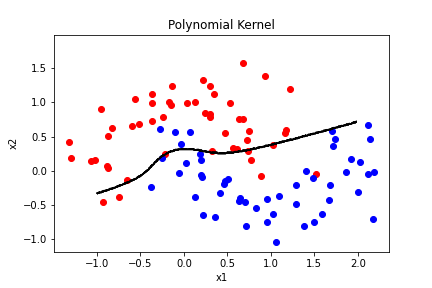
\includegraphics[width=\linewidth]{fig10.png}
					\label{fig:svc-poly}
				\end{subfigure}
				\begin{subfigure}[h!]{1\textwidth}
					\centering
					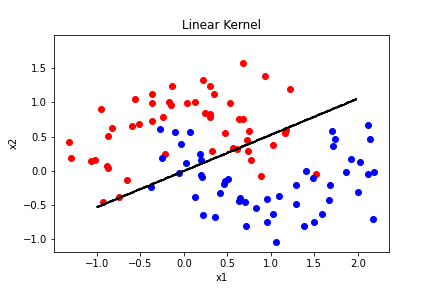
\includegraphics[width=\linewidth]{fig11.png}
					\label{fig:svc-linear}
				\end{subfigure}
				%\caption{Diferentes escolhas de \textit{Kernel}}
				\label{fig:kernel}
			\end{figure}
		\end{column}
	\end{columns}
	


\end{frame}

%\subsection{SVM}


%\subsection{Sistemas de otimização em tempo-real} % A subsection can be created just before a set of slides with a common theme to further break down your presentation into chunks

%\begin{frame}
%	\frametitle{Motivação}
%	\begin{itemize}
%		\item O custo de equipamentos para operação de uma mina gira em torno de centenas de milhões de dólares 
%		\item Um investimento deste tamanho necessita que eles sejam utilizados da melhor forma ao longo do tempo, de forma que os custos de operação sejam minimizados e a sua utilização maximizada
%		\item A manutenção da frota de caminhões de transporte é um dos maiores custos envolvidos, podendo atingir 100 milhões de dólares anualmente
%		\item Logo, o uso de modelos de otimização para encontrar a melhor utilização da frota que minimize os custos de manutenção possui grande potencial de redução nos custos da operação
%	\end{itemize}
%\end{frame}
%
%\begin{frame}
%	\frametitle{Objetivo}
%	\begin{itemize}
%		\item Implementar o modelo de otimização da programação de frota de caminhões em minas de céu aberto através da minimização do custo da manutenção presente na literatura proposto em \cite{topal2010a}
%	\end{itemize}
%\end{frame}
%
%%------------------------------------------------
%\section{Metodologia}
%%------------------------------------------------
%\subsection{Formulação do Problema}
%\begin{frame}
%	\frametitle{Definições preliminares}
%	\begin{columns}[c] % The "c" option specifies centered vertical alignment while the "t" option is used for top vertical alignment
%		
%		\column{.45\textwidth} % Left column and width
%		\begin{small}
%			\begin{table}[h!]
%				\begin{tabular}{p{0.5cm}p{1.5in}}
%					\multicolumn{2}{l}{\textbf{Índices}}                                                            \\                           
%					$t$                & Identificador do caminhão            \\
%					$b$                & Faixas de idade           \\
%					$y$                & Período de tempo (anos)   \\
%					$c$                & Faixa de operação crítica \\ & \\
%					\multicolumn{2}{l}{\textbf{Variáveis de decisão}}                                                            \\
%					$X_{t,b,y}$ & Número de horas alocadas para o caminhão $t$, faixa de idade $b$ no $y$-ésimo período de tempo \\
%					$Y_{t,b,y}$ & 1, se o caminão $t$ na faixa $b$ utilizou todas as horas disponíveis no período de tempo $y$                                      
%				\end{tabular}
%			\end{table}
%		\end{small}
%		\column{.55\textwidth} % Right column and width
%			\begin{small}
%				\begin{table}[h!]
%				\begin{tabular}{p{0.5cm}p{2in}}
%					\multicolumn{2}{l}{\textbf{Parâmetros}}                                                                                             \\
%					$C_{t,b,y}$        & Custo de manutenção (\$/hora) 
%					para um caminhão $t$ na faixa $b$ no $y$-ésimo período de tempo \\
%					$FE_t$               & Custo de reparo do motor do caminhão $t$                                                     \\
%					$A_{t,y}$          & Horas disponíveis do caminhão $t$ no período de tempo $y$                                      \\
%					M                   & Tamanho da faixa de idade (horas)                                                          \\
%					$R_y$                & Total de horas de operação para um período de tempo $y$ \\
%					$I_t$ & Idade inicial dos caminhão $t$ \\                                 
%				\end{tabular}
%			\end{table}
%		\end{small}
%		
%	\end{columns}
%\end{frame}	
%
%\begin{frame}
%\frametitle{Formulação}
%
%\textbf{Minimizar}
%\begin{equation}
%	\sum_{y \in Y}^{}\sum_{t \in T}^{}\sum_{b \in B}^{}X_{t,b,y}C_{t,b,y} + \sum_{y \in Y}^{}\sum_{t \in T}^{}Y_{t,c,y}FE_t 
%\end{equation}
%\end{frame}
%
%\begin{frame}
%	\frametitle{Formulação}
%	\textbf{Sujeito a}
%	\begin{small}
%		\begin{align}
%		&	\sum_{b \in B}^{}X_{t,b,y} \leq A_{t,y},\: \: \forall t \in T \:, \: \forall y\in Y \\
%		&	\sum_{y \in Y}^{}X_{t,b,y} \leq M,\: \forall t \in T \:, \forall b \in B \\
%		&	\sum_{k=1}^{y}X_{t,b,y} \geq MY_{t,b,y},\: \forall t \in T \:, \forall b \in B, \: \forall y\in Y \\
%		&	X_{t,(b+1),y} \geq M \sum_{k=1}^{y}Y_{t,b,k},\: \forall t \in T \:, \forall b \in B, \: \forall y\in Y \\
%		&	\sum_{t \in T}^{}\sum_{b \in B}^{}X_{t,b,y} = R_y ,\: \forall y \in Y \\
%		&	\sum_{y \in Y}^{}\sum_{b \in B}^{}X_{t,b,y} \leq Mb_{max} - I_t ,\: \forall t \in T 
%		\end{align}
%	\end{small}
%\end{frame}
%
%\subsection{Geração das instâncias}
%\begin{frame}
%	\frametitle{Geração das instâncias}
%	\begin{itemize}
%		\item Analisando as informações contidas em \cite{topal2010a}, constatou-se que os dados de disponibilidade e custo de manutenção dos caminhões estão incompletos, de forma que a instância executada pelo autor não possa ser replicada.
%		\item Infelizmente, os dados de custo de manutenção e de planejamento de longo prazo também não estavam disponíveis para minas reais
%		\item Então optou-se por gerar alguns destes valores de forma artificial, seguindo as recomendações da literatura
%	\end{itemize}
%\end{frame}
%
%
%\begin{frame}
%	\frametitle{Disponibilidade e idade dos caminhões}
%	\begin{block}{Disponibilidade}
%		\begin{equation}
%			A_{t,y} \sim \mathcal{U}_{[0.9, 0.95]} * 365 * 24
%			\label{eq:disp}
%		\end{equation}
%	\end{block}
%
%	\begin{block}{Idade dos caminhões}
%		\begin{equation}
%			I_{t} \sim \mathcal{U}_{[0, 20000]} 
%			\label{eq:it}
%		\end{equation}
%	\end{block}
%\end{frame}
%
%\begin{frame}
%	\frametitle{Produção anual}
%	\begin{block}{Produção anual}
%		\begin{equation}
%			R_y \sim \mathcal{U}_{[0.7, 0.8]} * 365 * 24 * t_{max}
%			\label{eq:prod}
%		\end{equation}
%	\end{block}
%
%%	\begin{figure}[h!]
%%		\centering
%%		\includegraphics[width=3.0in]{prod_targets.png}
%%		\caption{Exemplo de produção anual}
%%		\label{fig:prod_targets}
%%	\end{figure}
%\end{frame}
%
%\begin{frame}
%	\frametitle{Custo de manutenção}
%	\begin{itemize}
%		\item Os custos de manutenção variam de forma não-linear de acordo com a idade do caminhão e tendem a aumentar até um ponto onde um grande reparo é necessário \cite{nakousi2018}
%	\end{itemize}	
%
%%	\begin{figure}[h!]
%%		\centering
%%		\includegraphics[width=0.7\linewidth]{custos_manutencao.png}
%%		\caption{Exemplo de curva de custos de manutenção em função da idade}
%%		\label{fig:custo_manut}
%%	\end{figure}
%
%\end{frame}
%
%\subsection{Método de solução}
%
%\begin{frame}
%	\frametitle{Método de solução}
%	\begin{itemize}
%		\item Como foi formulado um problema de programação linear inteiro de larga escala e com muitas restrições, ele será resolvido utilizando o algoritmo Branch \& Cut com o CPLEX
%		\item Implementado na linguagem de programação Python versão 3.7.7
%		\item Executado em um notebook com Intel Core i7 Quad Core 2.4GHz, 8GB de memória RAM
%	\end{itemize}
%\end{frame}
%
%
%\subsection{Desenho do experimento}
%
%\begin{frame}
%	\frametitle{Desenho do experimento}
%	O algoritmo será avaliado sobre 4 instâncias distintas do problema.	O número de faixas de idade será igual a 20 para todas as instâncias.
%	\begin{table}[h!]
%	\caption{Valores de cada instância gerada}
%	\label{tab:instances}
%	\centering
%	\begin{tabular}{l|c|c|c|c|}
%		\cline{2-5}
%		& \textbf{Pequena} & \textbf{Média} & \textbf{Grande} & \textbf{Artigo} \\ \hline
%		\multicolumn{1}{|l|}{\textbf{Caminhões}} & 5                & 20             & 45              & 34              \\ \hline
%		\multicolumn{1}{|l|}{\textbf{Anos}}      & 3                & 5              & 10              & 10              \\ \hline
%		\multicolumn{1}{|l|}{\textbf{M}}         & 2000             & 4000           & 5000            & 5000            \\ \hline
%		\multicolumn{1}{|l|}{\textbf{Idade crítica}}         & 16000             & 40000           & 75000            & 	75000            \\ \hline
%	\end{tabular}
%	\end{table}
%	Na instância \textbf{Artigo}, serão considerados os valores disponíveis em \cite{topal2010a} para objetivos de produção, número de caminhões e suas respectivas idades inicias.
%	
%
%\end{frame}	
%
%\section{Resultados}
%
%\subsection{Pequena}
%\begin{frame}
%	\frametitle{Pequena}
%	\begin{itemize}
%		\item Um total de 480 variáveis de decisão e 567 restrições foram criadas para esta instância e o esforço computacional foi bem baixo para a sua solução, uma vez que o CPLEX encontrou o ótimo global em menos de 0.5 segundos.
%		\item As idades iniciais foram definidas como [0, 0, 8000 e 8000] e uma produção de 25000 horas por ano.
%	\end{itemize}
%\end{frame}
%
%
%
%%\begin{frame}
%%	\frametitle{Média}
%%	\begin{figure}[h!]
%%		\centering
%%		\includegraphics[width=0.8\linewidth]{average_solution_values.png}
%%		\caption{Alocação de horas por caminhão em cada ano para a instância média. Os valores estão em múltiplos de 1000 horas.}
%%		\label{fig:average_solution_values}
%%	\end{figure}
%%\end{frame}
%%
%%\begin{frame}
%%	\frametitle{Média}
%%	\begin{figure}[h!]
%%		\centering
%%		\includegraphics[width=0.8\linewidth]{average_solutions_bins.png}
%%		\caption{Alocação de horas por caminhão em cada faixa de idade para a instância média}
%%		\label{fig:average_solutions_bins}
%%	\end{figure}
%%\end{frame}
%
%
%\subsection{Grande}
%
%\begin{frame}
%	\frametitle{Grande}
%	\begin{itemize}
%		\item Total de 18000 variáveis de decisão e 18955 restrições
%		\item CPLEX conseguiu chegar ao gap relativo de 1\% em cerca de 3.5 minutos
%	\end{itemize}
%\end{frame}
%
%%\begin{frame}
%%	\frametitle{Grande}
%%	\begin{figure}[h!]
%%		\centering
%%		\includegraphics[width=0.8\linewidth]{large_solution_accumulated.png}
%%		\caption{Idade dos caminhões ao longo dos anos. Os valores estão em múltiplos de 1000 horas.}
%%		\label{fig:large_solution_accumulated}
%%	\end{figure}
%%\end{frame}
%%
%%\begin{frame}
%%	\frametitle{Grande}
%%	\begin{figure}[h!]
%%		\centering
%%		\includegraphics[width=0.8\linewidth]{large_solution_values.png}
%%		\caption{Alocação de horas por caminhão em cada ano para a instância grande. Os valores estão em múltiplos de 1000 horas.}
%%		\label{fig:large_solution_values}
%%	\end{figure}
%%\end{frame}
%
%\begin{frame}
%	\frametitle{Artigo}
%	\begin{itemize}
%		\item Total de 13600 variáveis de decisão e 14324 restrições
%		\item Com parâmetros padrão, o CPLEX executou durante 30 minutos para chegar a um gap relativo de 6.40\%
%		\item Ajustando a estratégia de \textit{probing} para o nível mais agressivo, o parâmetro de ênfase  para priorizar a otimalidade e ativando a heurística de busca local, executando o algoritmo por 30 minutos, foi possível chegar a um gap de 5.76\%.
%	\end{itemize}
%\end{frame}
%
%
%%------------------------------------------------
%
%
%\section{Conclusão}
%\begin{frame}
%	\frametitle{Conclusão}
%	\begin{itemize}
%		\item Implementado um MILP para otimização da programação de equipamentos de mina de céu aberto proposto na literatura \cite{topal2010a}
%		\item Para as 3 instâncias artificias, o CPLEX não teve grandes dificuldades para a sua solução. 
%		\item Entretanto, para dados mais próximos da realidade, foi notável o quão mais difícil o problema se tornou
%		\item A maior dificuldade do trabalho consistiu na geração dos dados artificias e no entendimento das equações da formulação disponível na literatura
%	\end{itemize}
%\end{frame}


%------------------------------------------------
%------------------------------------------------

%\begin{frame}
%\frametitle{Theorem}
%\begin{theorem}[Mass--energy equivalence]
%$E = mc^2$
%\end{theorem}
%\end{frame}
%
%%------------------------------------------------
%
%\begin{frame}[fragile] % Need to use the fragile option when verbatim is used in the slide
%\frametitle{Verbatim}
%\begin{example}[Theorem Slide Code]
%\begin{verbatim}
%\begin{frame}
%\frametitle{Theorem}
%\begin{theorem}[Mass--energy equivalence]
%$E = mc^2$
%\end{theorem}
%\end{frame}\end{verbatim}
%\end{example}
%\end{frame}
%
%%------------------------------------------------
%
%\begin{frame}
%\frametitle{Figure}
%Uncomment the code on this slide to include your own image from the same directory as the template .TeX file.
%%\begin{figure}
%%\includegraphics[width=0.8\linewidth]{test}
%%\end{figure}
%\end{frame}
%
%%------------------------------------------------
%
%\begin{frame}[fragile] % Need to use the fragile option when verbatim is used in the slide
%\frametitle{Citation}
%An example of the \verb|\cite| command to cite within the presentation:\\~
%
%This statement requires citation \cite{p1}.
%\end{frame}

%------------------------------------------------

\begin{frame}
\frametitle{Referências}
\footnotesize{
\begin{thebibliography}{99} % Beamer does not support BibTeX so references must be inserted manually as below
% APA
\bibitem[Vapnik, 1992]{vapnik}
Boser, B. E., Guyon, I. M., \& Vapnik, V. N. (1992, July). A training algorithm for optimal margin classifiers. In Proceedings of the fifth annual workshop on Computational learning theory (pp. 144-152).
\bibitem[Haykin, 2007]{haykin}
Haykin, S. (2007). Neural Networks: A Comprehensive Foundation (3rd Edition).
\bibitem[Cover, 1965]{cover}
Cover, T. M. (1965). Geometrical and statistical properties of systems of linear inequalities with applications in pattern recognition. IEEE transactions on electronic computers, (3), 326-334.
\bibitem[Mercer, 1909]{mercer}
Mercer, J. (1909). Xvi. functions of positive and negative type, and their connection the theory of integral equations. Philosophical transactions of the royal society of London. Series A, containing papers of a mathematical or physical character, 209(441-458), 415-446.

\end{thebibliography}
}
\end{frame}

%------------------------------------------------

\begin{frame}
\Huge{\centerline{Obrigado!}}
\end{frame}

%----------------------------------------------------------------------------------------

\end{document} 